\documentclass[../IoMusT.tex]{subfiles}
\begin{document}
\subsection{Sistemul de operare Raspbian}

\subsection{Protocolul de comunicare MIDI}
\subsubsection{Prezentarea mesajelor MIDI}
% reformulare tastatura
% de completat alte tipuri de mesaje
Comunicarea între un instrument muzical electric și un calculatori se întâmplă de cele mai multe ori printr-un protocol de comunicare numit MIDI (Digital Interface for Musical Interface). Prin acest protocol putem trimite sau primi date de la instrumentul respectiv sub forma unor mesaje MIDI, fiecare astfel de mesaj fiind o instrucțiune. Putem să ne gândim la ele ca fiind o altfel de partitură în care sunt marcate înălțimea și puterea (velocitatea) cu care notele muzicale au fost cântate. Aceste date primite se pot reda audio sau se pot chiar modifica facând acest tip de comunicare un instrument puternic în industria muzicală. 
\\
\par Un mesaj MIDI constă dintr-un octet de stare, care indică tipul mesajului, urmat de până la doi octeți de date care conțin parametrii. Tipul mesajului poate fi de mai multe feluri, acestea variând de la un instrument la altul. Principalele tipuri de mesaje sunt cele de NOTE ON sau NOTE OFF, care indică faptul că interpretul a atins tastatura muzicală respectiv cănd s-a dat drumul la tastă. Diferența de timp dintre aceste două tipuri ne poate da timpul în care a fost ținută o notă muzicală. Cu toate că aceste mesaje sunt unele standard trebuie avut în vedere că nu fiecare instrument poate genera astfel de mesaje. Instrumentele mai vechi au o gamă mai închisă in ceea ce privește multitudinea de tipuri de mesaje ce pot trimite.
\\ 
\par Parametrii unui mesaj MIDI, după cum s-a discutat și în primul paragraf, pot conține nota muzicală și velocitatea cu care aceasta a fost cântată. Reprezentarea acestei note muzicale se face printr-un număr de la 0 pana 127 \cite{MidiSoftware}, 0 fiind nota cea mai joasă cu cea mai mică frecvență. Astfel de exemplu numărul 60 se asociază notei Do cu frecvența 261.63. Puterea cu care nota respectivă a fost apăsată se caracterizează printr-un număr de la 1 la 127 \cite{MidiSoftware}, o apăsare decentă (fără prea multă forță) fiind aproximativ 64. Datorită faptului că pianul folosit în acest proiect are o reprezentare imprecisă a acestui număr, în aplicație ne vom folosi numai numărul notei MIDI din care vom calcula frecvența, folosind o formulă, cu care trebuie să vibreze motoarele când o clapă e apăsată. Când vine vorba despre programarea acestor mesaje, modul în care sunt reprezentate depinde de librăria folosită în limbajul de programare respectiv. Despre parsarea acestora vom detalia în subcapitolele ce urmează.

\subsection{Limbajul de programare Python}
\subsection{Prezentare generală}
Python este un limbaj de programare devenit foarte popular datorită faptului că este proiectat să fie ușor de învățat și de înțeles. Este un limbaj de scriptare ceea ce înseamnă că codul scris nu este compilat ci mai degrabă interpretat. Ca și celelalte limbaje de nivel înalt și Python suportă mai multe paradigme de programare cum ar fi programare procedurală, orientată pe obiect sau funcțională sprijinind astfel dezvoltarea unei game largi de aplicații. Poate fi folosit atât pentru realizarea proiectelor de dimensiuni mai mici cât și pentru cele mai mari, fiind cel mai des utilizat în crearea aplicațiilor web (este folosit de companiile Google și Yahoo!), științifice sau de divertisment, cum ar fi jocuri. Este foarte mult folosit și în proiectele ce țin de Internetul lucrurilor, având destule biblioteci ce pot fi folosite pentru programarea senzorilor și actuatorilor.
\\
\par Faptul că limbajul de programare Python oferă o gamă largă de biblioteci și extinderi, constituie un avantaj în programarea aplicațiilor complexe. Biblioteca standard a limbajului este deseori citat și ca unul dintre cele mai mari puncet forte ale sale, oferind multe tool-uri pentru difeite sarcini.
\\
\par Sintaxa și semantica limbajului de programare sunt concepute astfel încât codul să fie cât mai ușor de scris și de înțeles de către programator. Spre deosebire de alte limbaje de programare, Python nu folosește acolade pentru delimitarea blocurilor, aceste delimitări făcându-se cu ajutorul indentării. Un cod indenatat incorect va arunca eroare de tipul IndentationError. Se poate vedea în figura \ref{fig:indent} o bucată de cod indentat corect.
\begin{figure}[h]
\centering
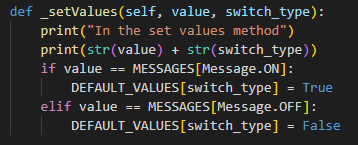
\includegraphics{indentare}
\caption{}
\label{fig:indent}
\end{figure}
O scăderii  a indentării  seminfică sfârșitul unui bloc curent în timp ce creșterea indică începerea unei noi afirmații. Un statement (afirmație) este o unitate sintactică a limbajelor de programare imperative care exprimă  unele acțiuni care trebuie efectuate.
\\
\par În Python, ca și în celelalte limbaje de programare, putem face diferența dintre o metodă și o funcție. Ambele trebuie să înceapă cu cuvântul cheie def urmat de denumirea funcției/metodei. Spre deosebire de alte limbaje de programare, în cazul metodelor în Python trebuie specificat explicit cuvântul self în parametrii metodei. Acest cuvânt indică instanța clasei de care aparține metoda respectivă.
% include duck typing

% include image from pinout
% add cleanup
\subsubsection{Biblioteca Gpiozero pentru programarea pinurilor}
Gpiozero este o bibliotecă care oferă o interfață simplă pentru programarea GPIO-urilor de pe placa de dezvoltare Raspberry Pi. Spre deosebire de alte biblioteci, aceasta oferă o curbă de învățare mai lină pentru începători și posibilitatea dezvoltării proiectelor complicate cu mai multă ușurință și mai puține linii de cod. La început Gpiozero a fost doar un layout peste biblioteca RPi.GPIO, ulterior fiind adăugate diferite suporturi. În prezent RPi.GPIO este folosit ca bibliotecă implicită pentru Gpiozero, această configurație putând fii schimbată, existând ma multe astfel de biblioteci, cum ar fi de exemplu pigpio. Instalarea acestei biblioteci este necesară numai în cazul în care se folosește pe alt sistem de operare decât Raspbian, pe acesta fiind deja inclus. Odată cu instalarea ei putem rula comanda pinout din linia de comandă pentru a vedea vizual detalii despre pinii disponibili de pe Raspberry Pi. Acest lucru devine în ajutor în momentul în care, la configurarea pinurilor, trebuie să precizăm numărul pinului ales astfel fiind mult mai ușor de urmat poziționarea fiecărui pin în parte.
\\
\par În comparație cu alte biblioteci, în Gpiozero se pote observa o abordare orientată pe obiecte, acesta folosind clase în loc de funcții. Pe lângă niște clase specifice, Gpiozero oferă două clase mari de bază, InputDevice și OutputDevice, celelalte fiind derivate din acestea, fiecare având metode și proprietăți specifice care sunt adaptate dispozitivului controlat. Clasa OutputDevices și tot ce derivă din ea este folosită pentru controlarea dispozitivelor de ieșire cum ar fi de exemplu LED-urile, pe când cea de InputDevice este pentru dispozitivele care sunt folosite pentru a furniza date și semnale de control. Asftel alegerea clasei de lucru este mult mai vizibilă și mult mai ușoară.
\\
\par Pentru controlarea motoarelor de vibrații în proiectul de față s-au folosit clasa PWMOutputDevice derivat din OutputDevice care permit și modularea lățimii pulsului. Importarea bibliotecii se face simplu, conform figurei \ref{fig:import}.
\begin{figure}[h]
\centering
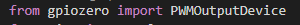
\includegraphics{importPWM}
\caption{Importare biblioteca Gpiozero}
\label{fig:import}
\end{figure}
Constructorul acestei clase are mai mulți parametrii, majoritatea dintre ei fiind setate în mod implicit. Singurul parametru obligatoriu este numărul pinului cu care dorim să lucrăm. Trebuie avut grijă pentru că numerotarea pinurilor de pe RaspberryPi se poate face in mai multe feluri, însă biblioteca Gpiozero folosește implicit numerotarea Broadcom.
\subsubsection{Folosirea bibliotecii Mido}
\subsubsection{Programarea asincrona cu biblioteca Asyncore}

\subsection{Limbajul de programare Java}
\subsubsection{Folosirea firelor de executie in Java}

\subsection{Sistemul de operare Android}
\subsubsection{Baza de date SQLite}
\end{document}